\begin{tcolorbox}
In diesem Kapitel werden erste Skizzen (Mockups) der Benutzeroberflächen dargestellt.
Diese sollen in erster Linie dazu dienen, dem Kunden einen Überblick über die zu erstellenden UIs zu geben und ggf. Änderungen frühzeitig durchführen zu können.
Dafür eignen sich spezielle Tools, wie z.B. Balsamiq Mockups\footnote{\url{https://balsamiq.com/products/mockups}}.
\end{tcolorbox}
\begin{figure}[h]
	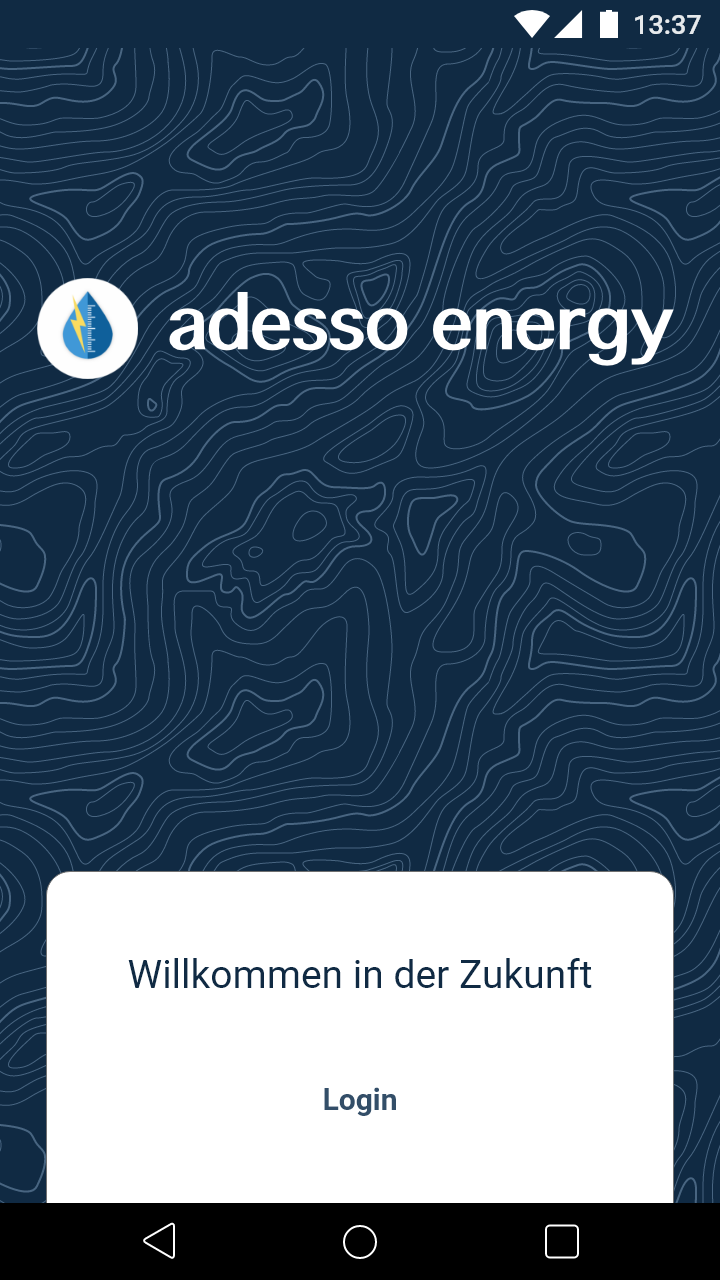
\includegraphics[scale = 0.22]{img/AndroidMockup/splash}	
	\caption{Startbildschirm}
	\label{fig:mock-start}

\end{figure}

\begin{figure}[h]
	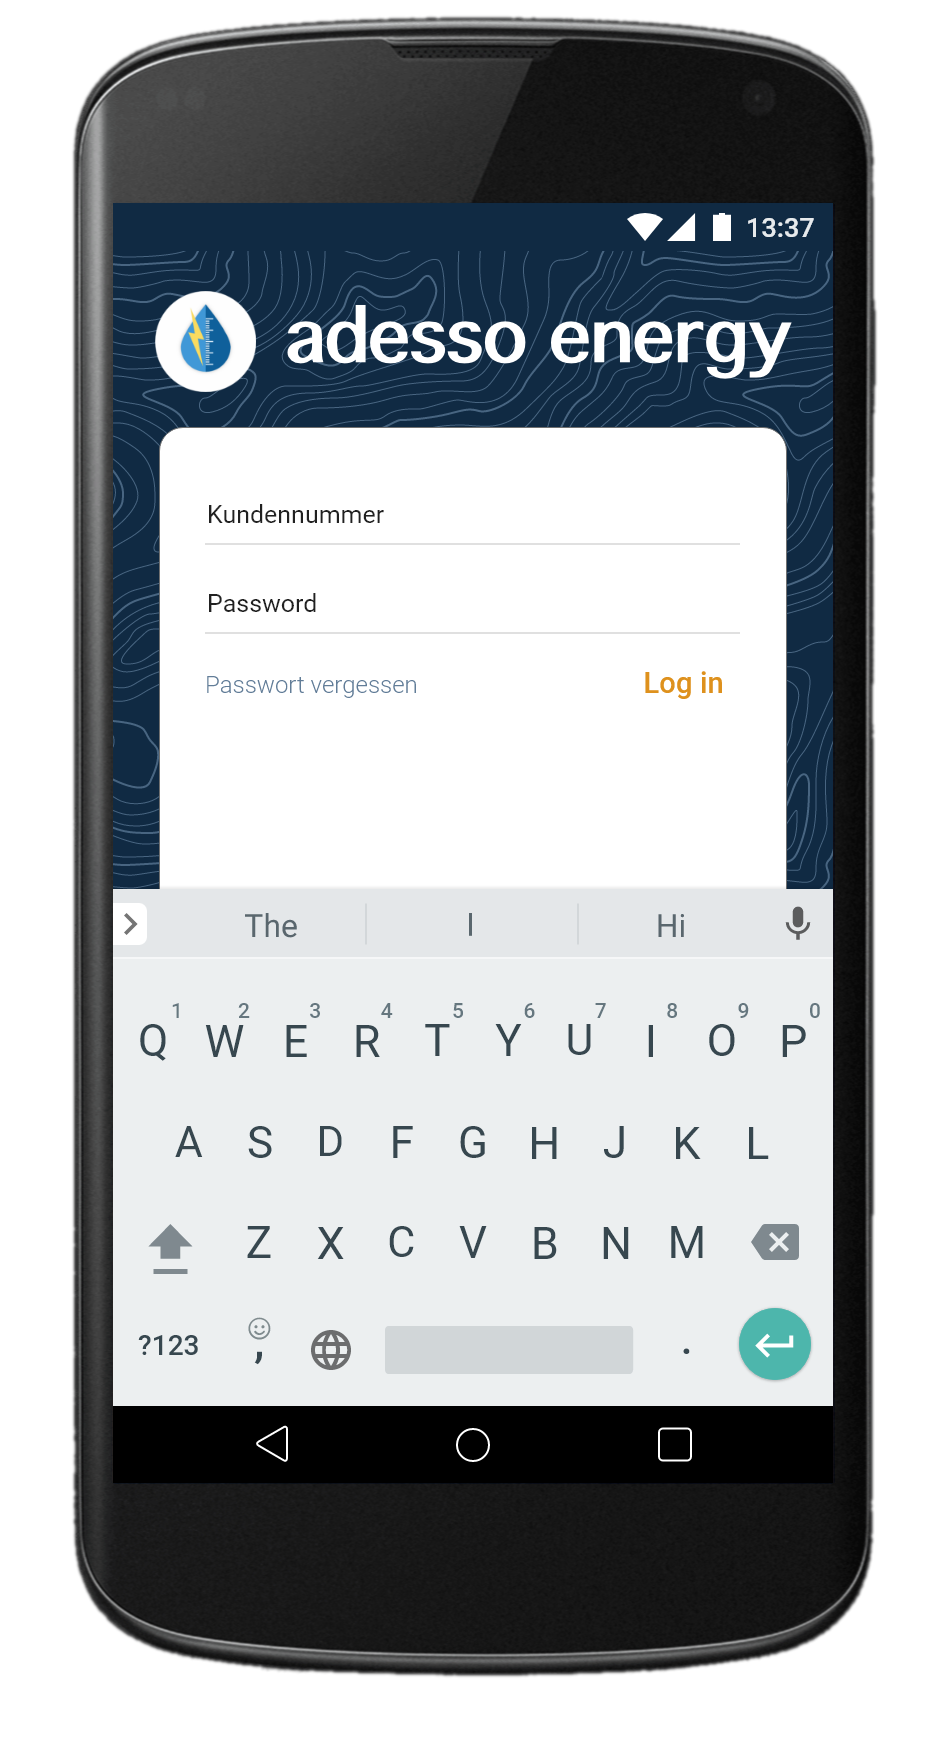
\includegraphics[scale = 0.22]{img/AndroidMockup/login}		
	\caption{Login}
	\label{fig:mock-pw}
\end{figure}

\begin{figure}[h]
	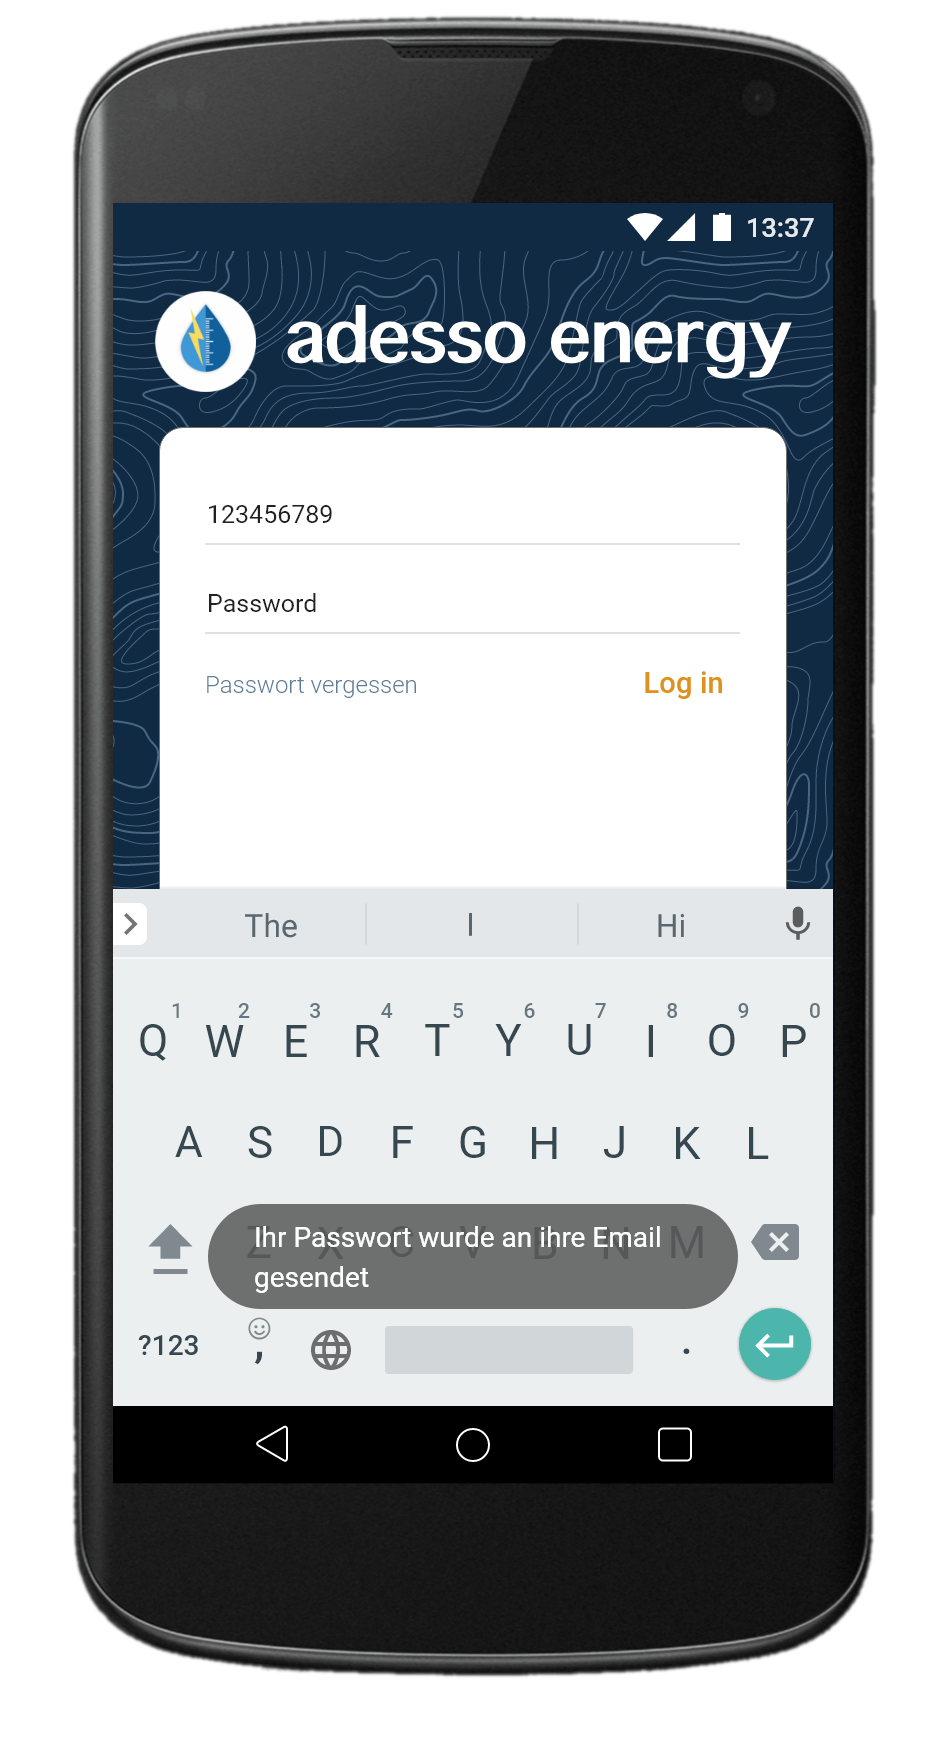
\includegraphics[scale = 0.22]{img/AndroidMockup/forgotPassword}		
	\caption{Passwort ändern}
	\label{fig:mock-pw}
\end{figure}

\begin{figure}[h]
	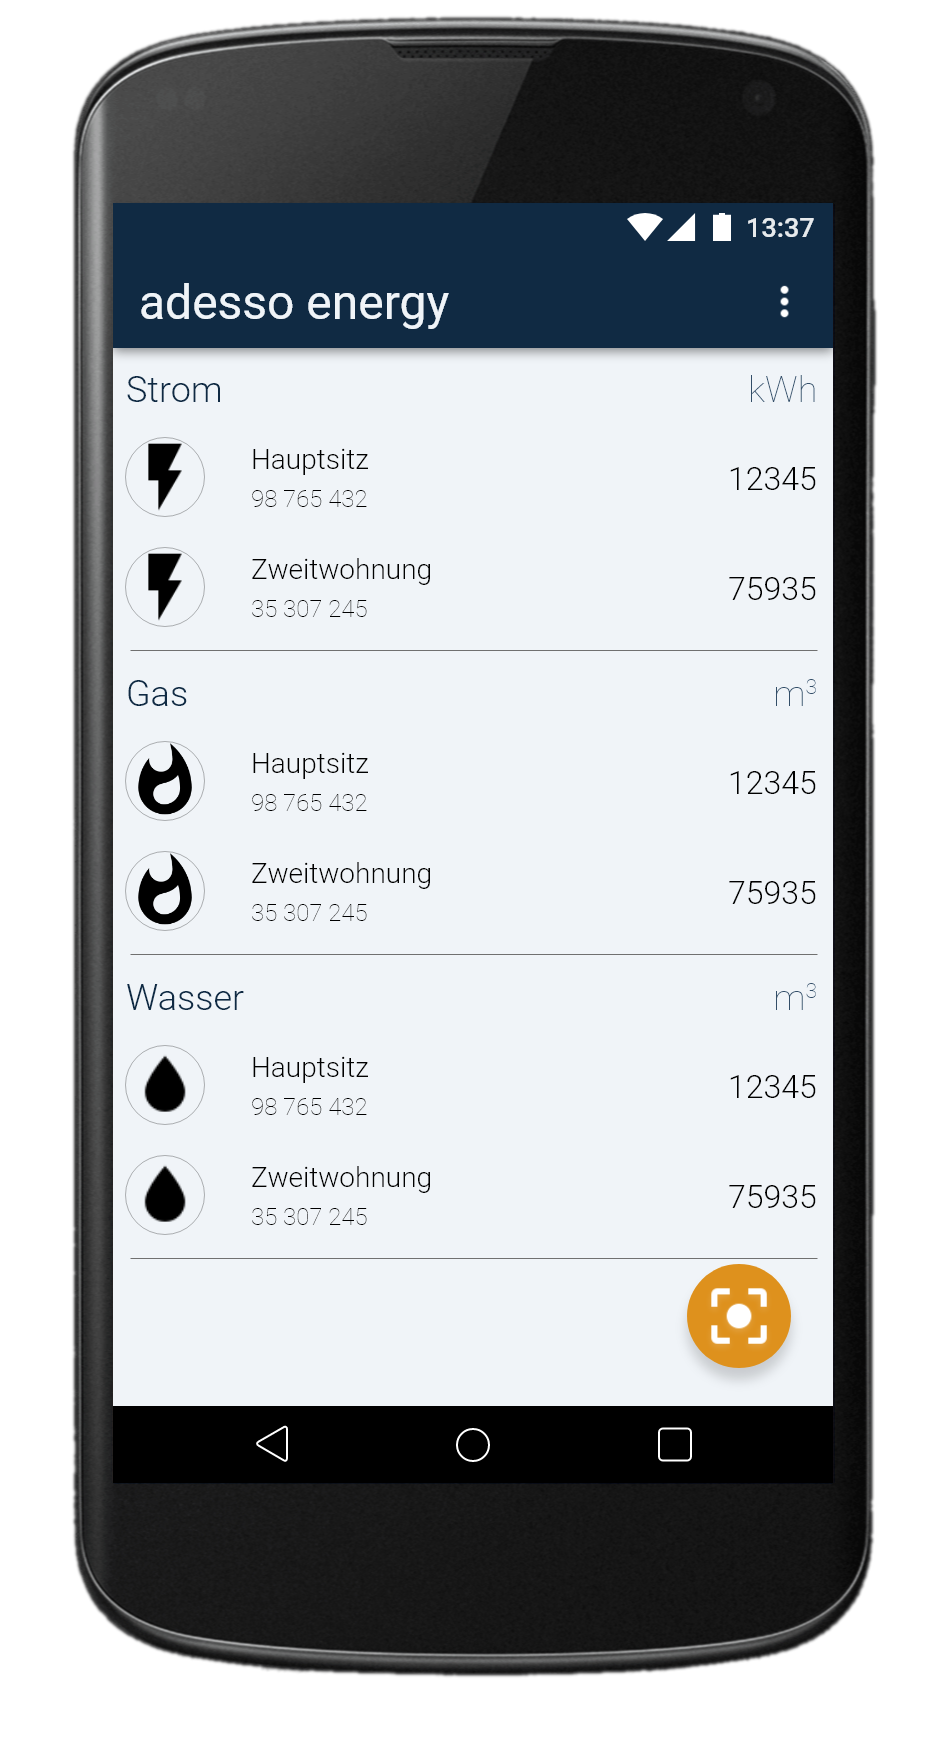
\includegraphics[scale = 0.22]{img/AndroidMockup/Main}		
	\caption{Hauptbildschirm}
	\label{fig:mock-pw}
\end{figure}

\begin{figure}[h]
	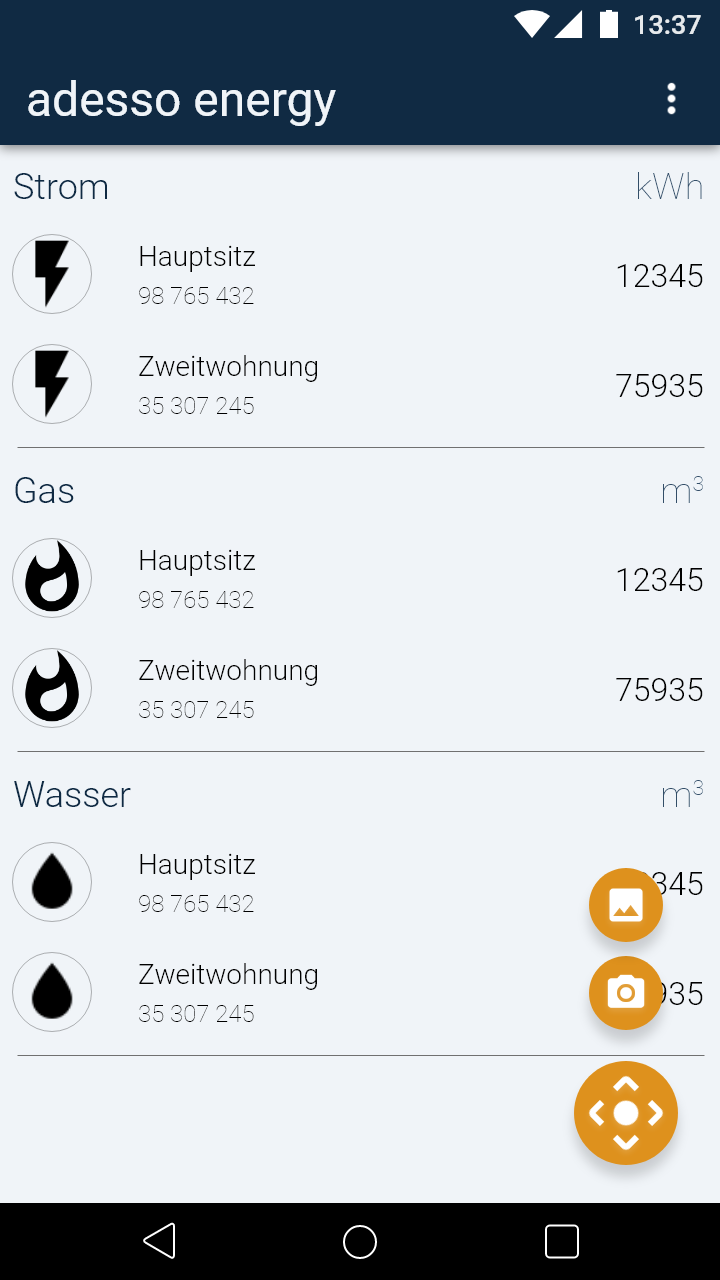
\includegraphics[scale = 0.22]{img/AndroidMockup/FABMenu}		
	\caption{FABMenü}
	\label{fig:mock-pw}
\end{figure}

\begin{figure}[h]
	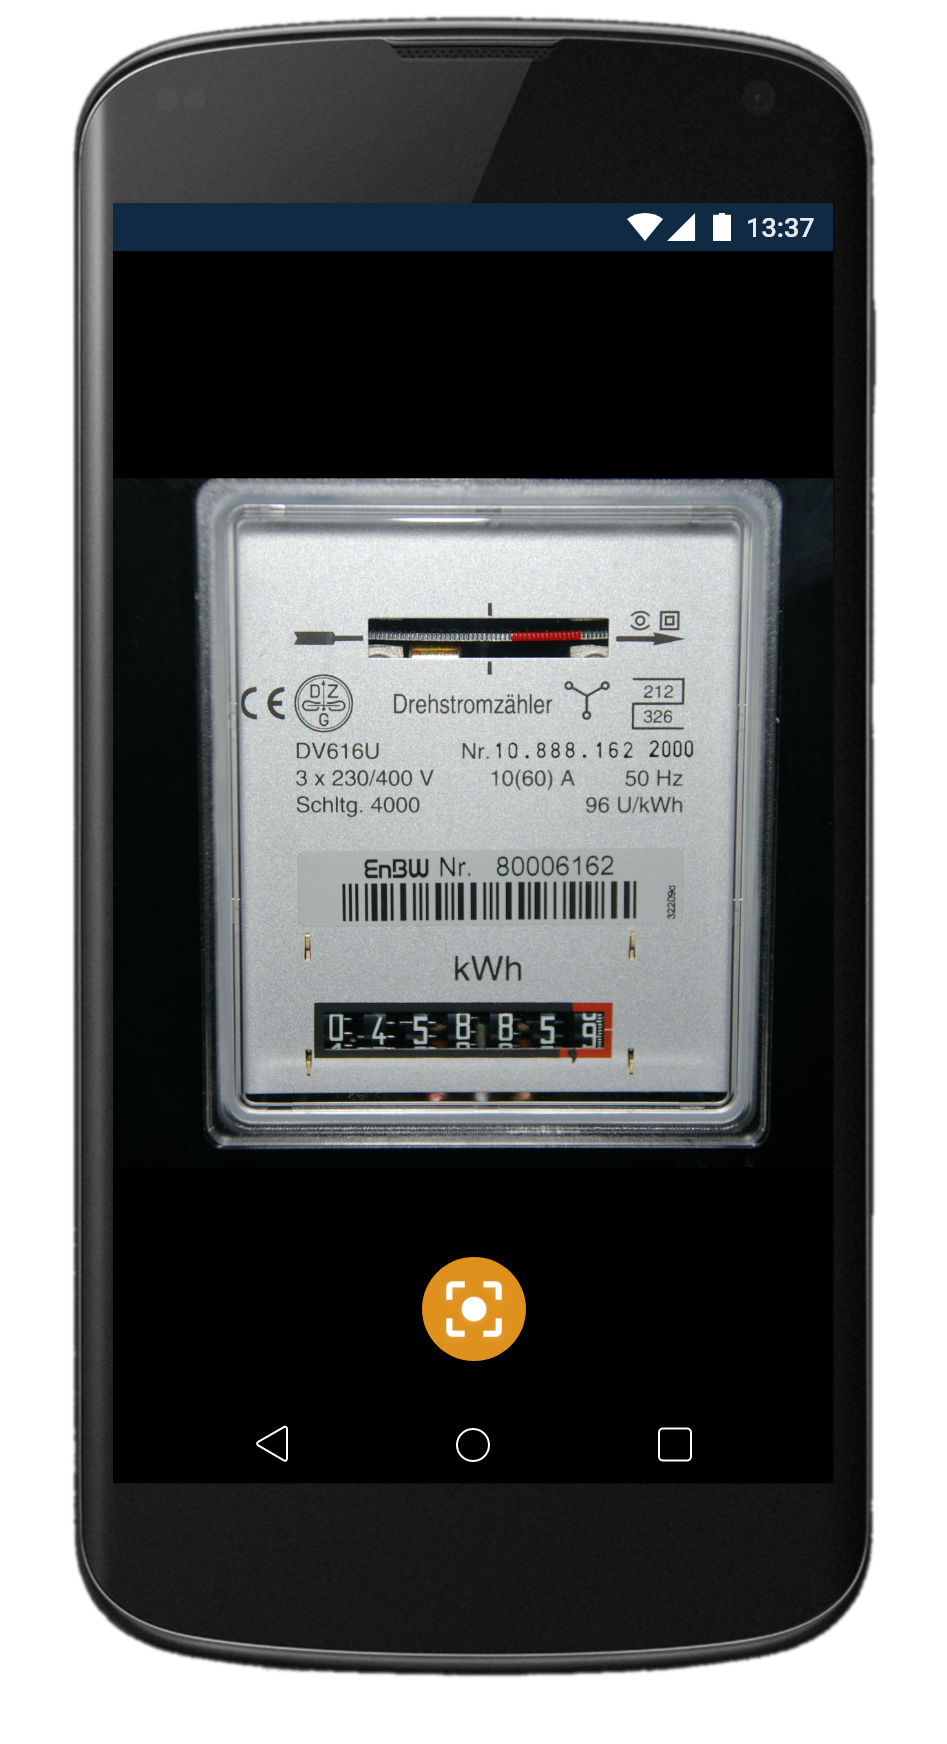
\includegraphics[scale = 0.22]{img/AndroidMockup/SystemCamera}		
	\caption{Kamera Perspektive}
	\label{fig:mock-pw}
\end{figure}

\begin{figure}[h]
	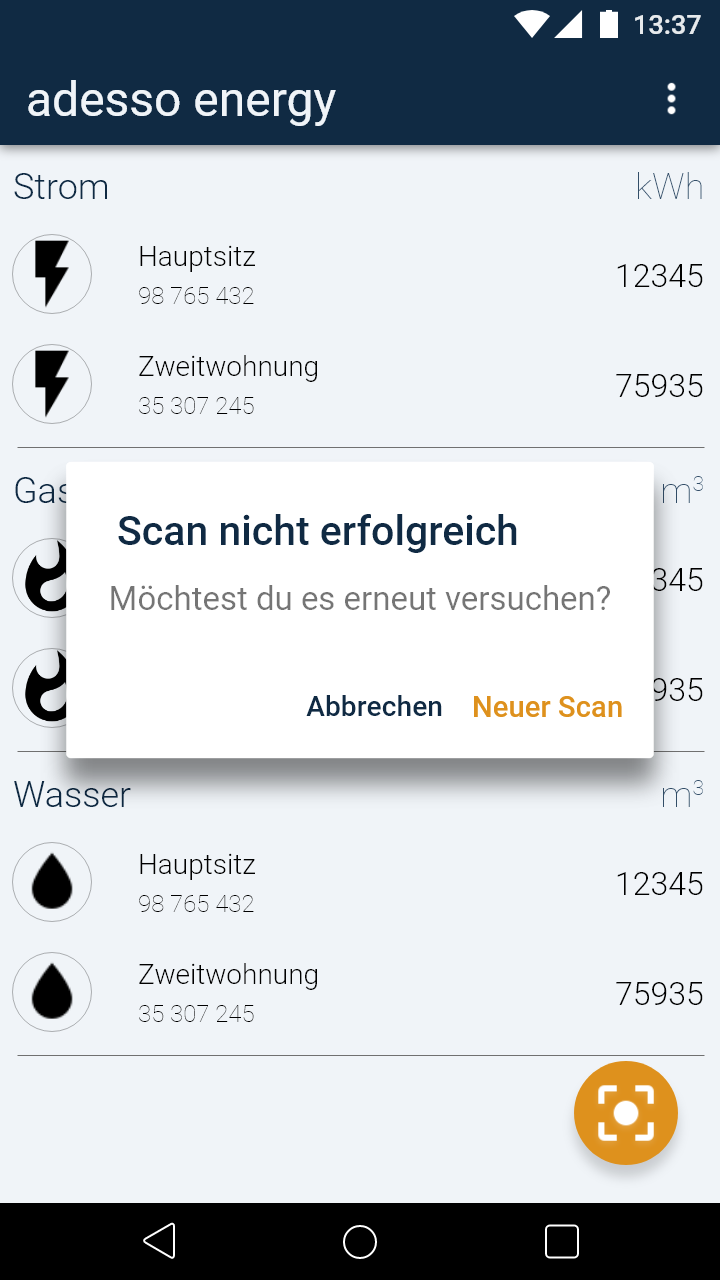
\includegraphics[scale = 0.22]{img/AndroidMockup/imageFailed}		
	\caption{Fehler beim Bild Scannen}
	\label{fig:mock-pw}
\end{figure}

\begin{figure}[h]
	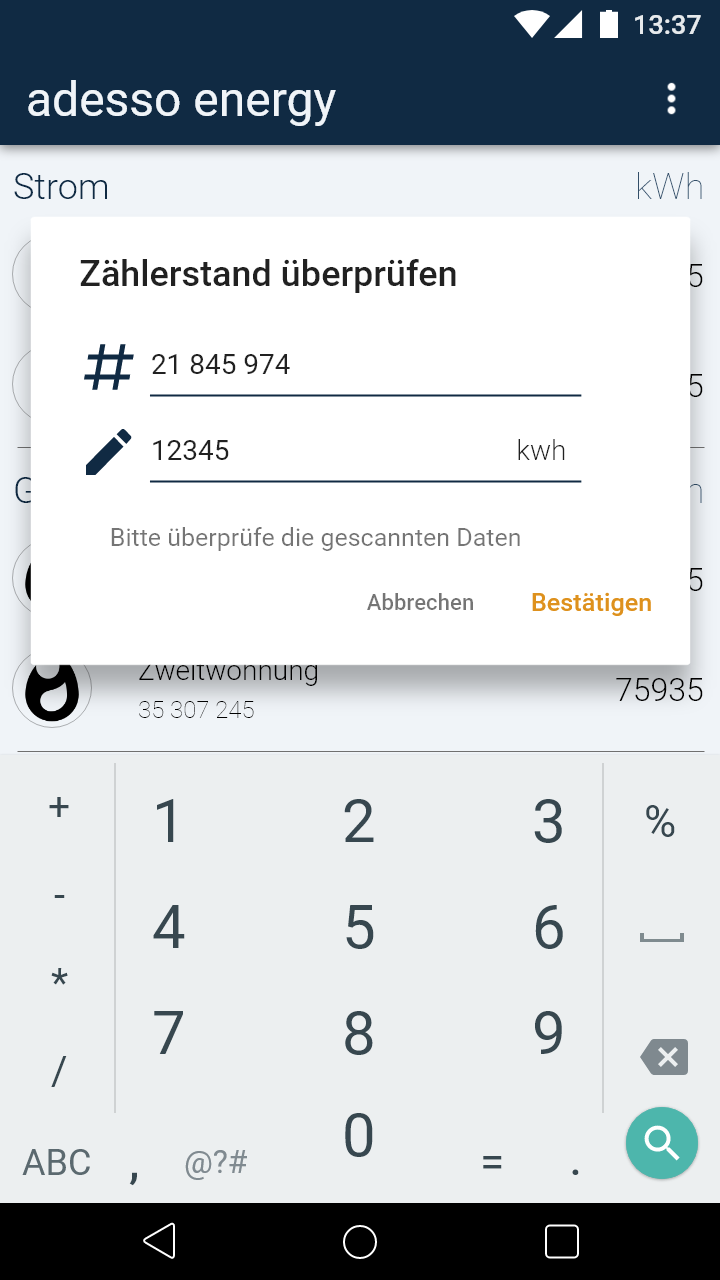
\includegraphics[scale = 0.22]{img/AndroidMockup/check}		
	\caption{Überprüfung der Zahlen}
	\label{fig:mock-pw}
\end{figure}

\begin{figure}[h]
	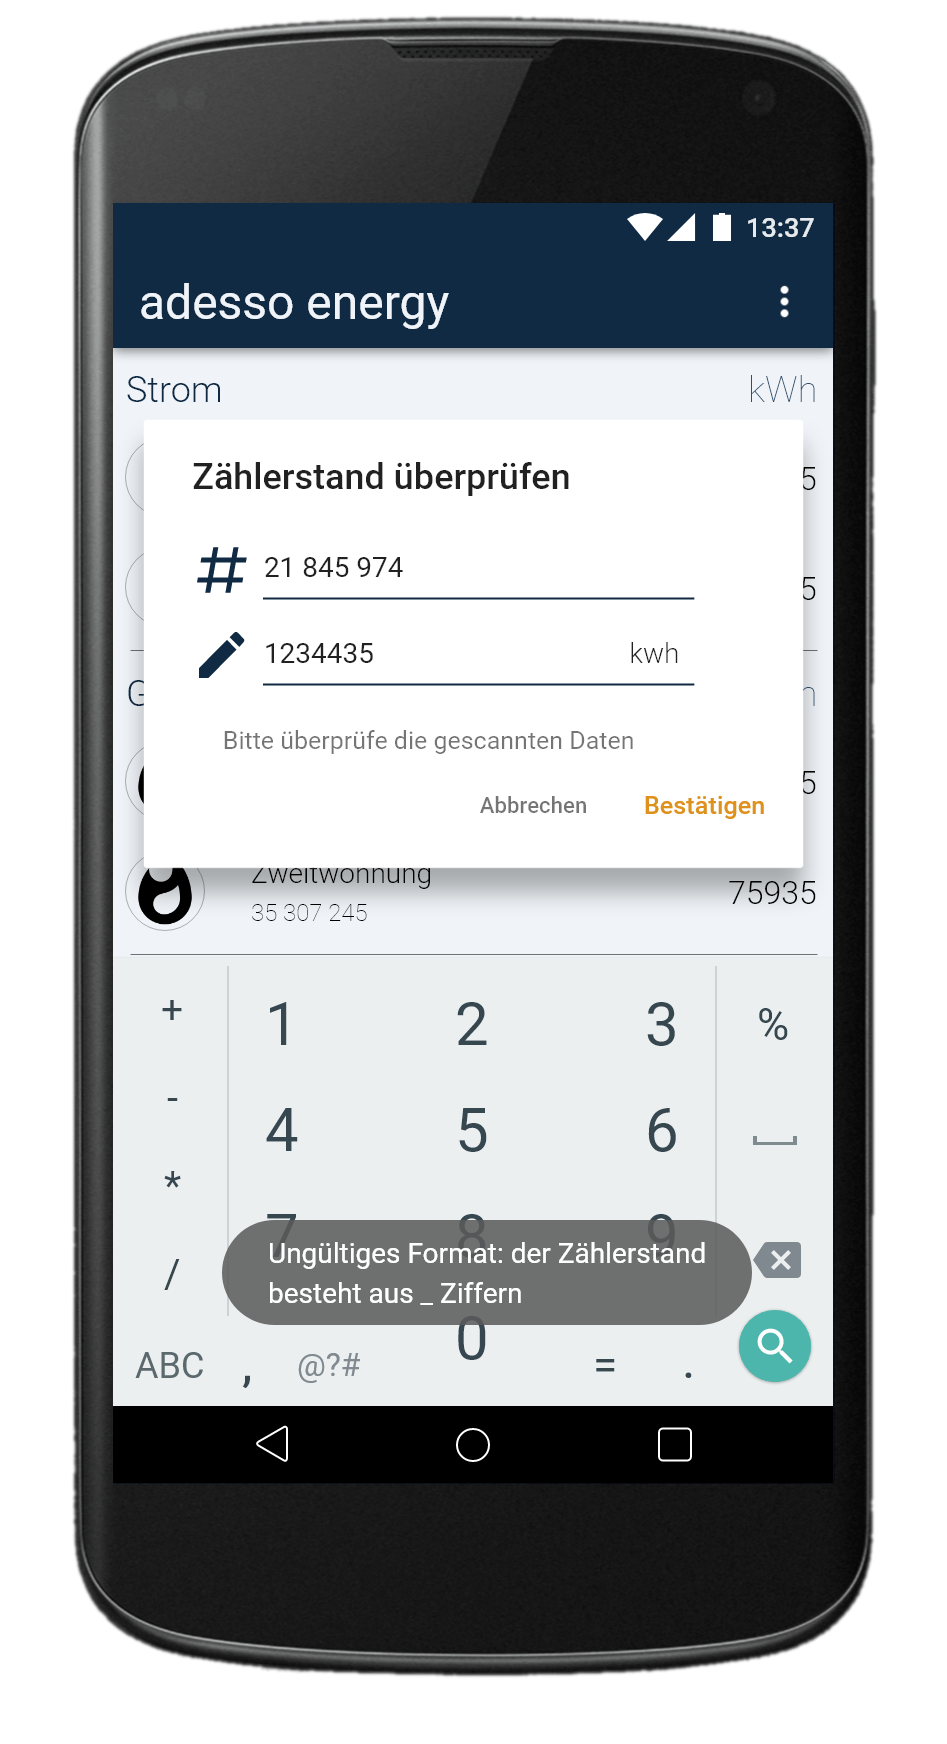
\includegraphics[scale = 0.22]{img/AndroidMockup/illegalFormatException}		
	\caption{Falsches Zahlenformat}
	\label{fig:mock-pw}
\end{figure}

\begin{figure}[h]
	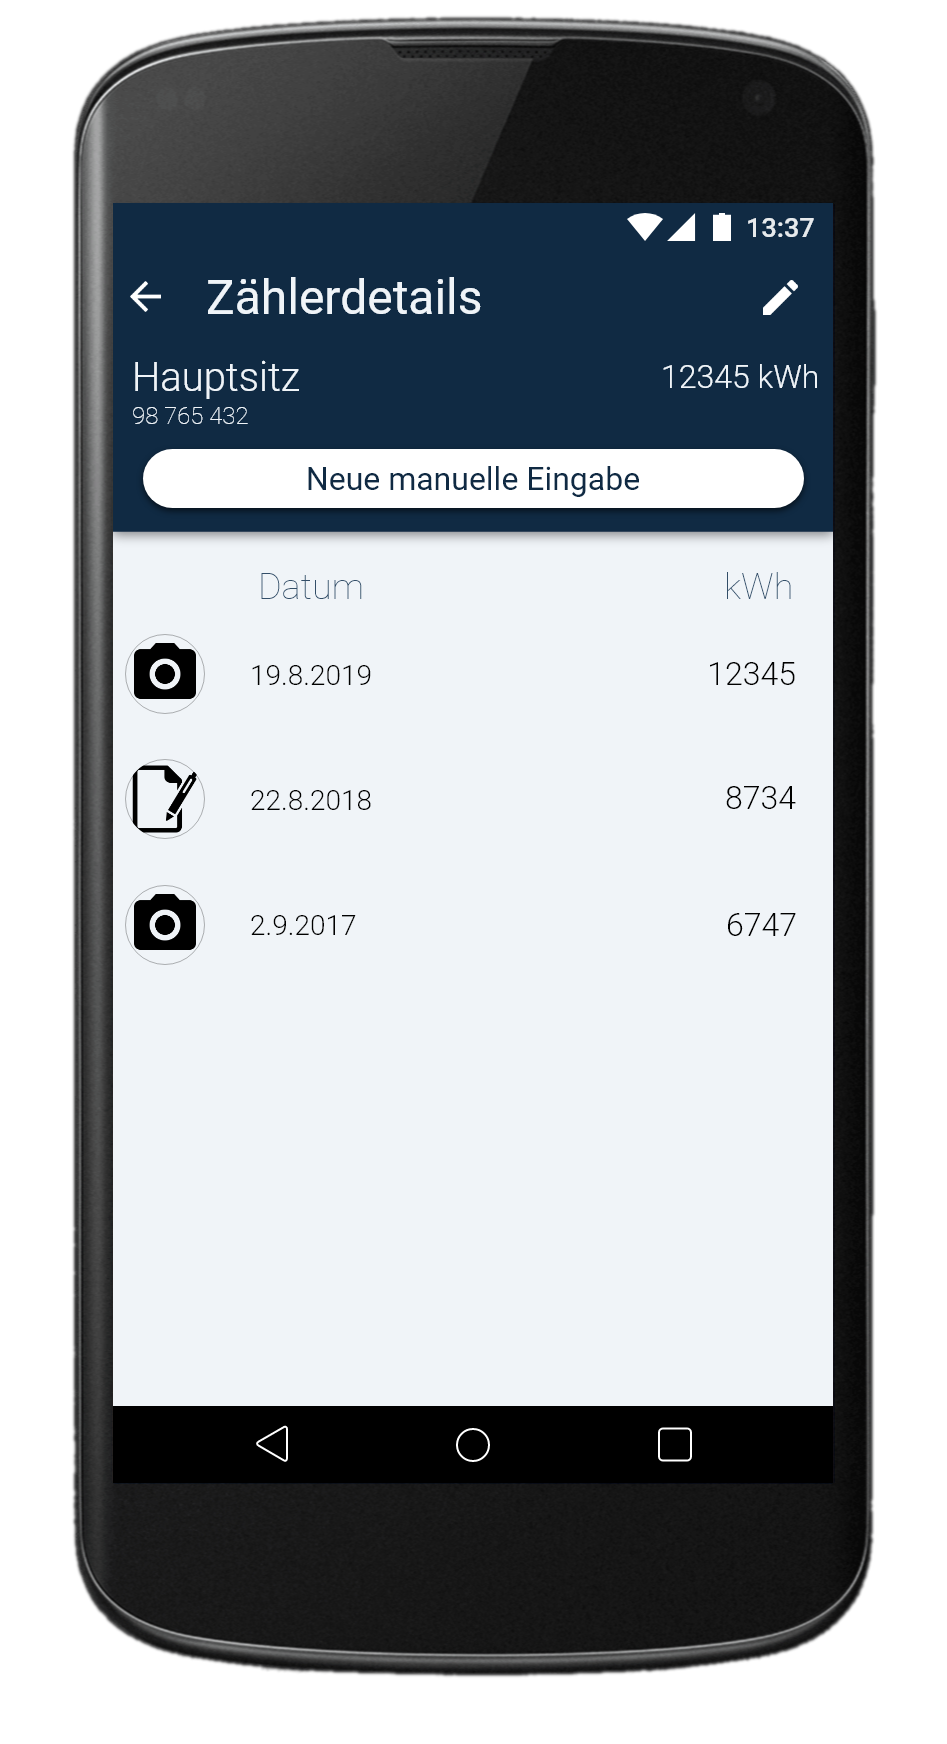
\includegraphics[scale = 0.22]{img/AndroidMockup/history}		
	\caption{Zählerstand History}
	\label{fig:mock-pw}
\end{figure}

\begin{figure}[h]
	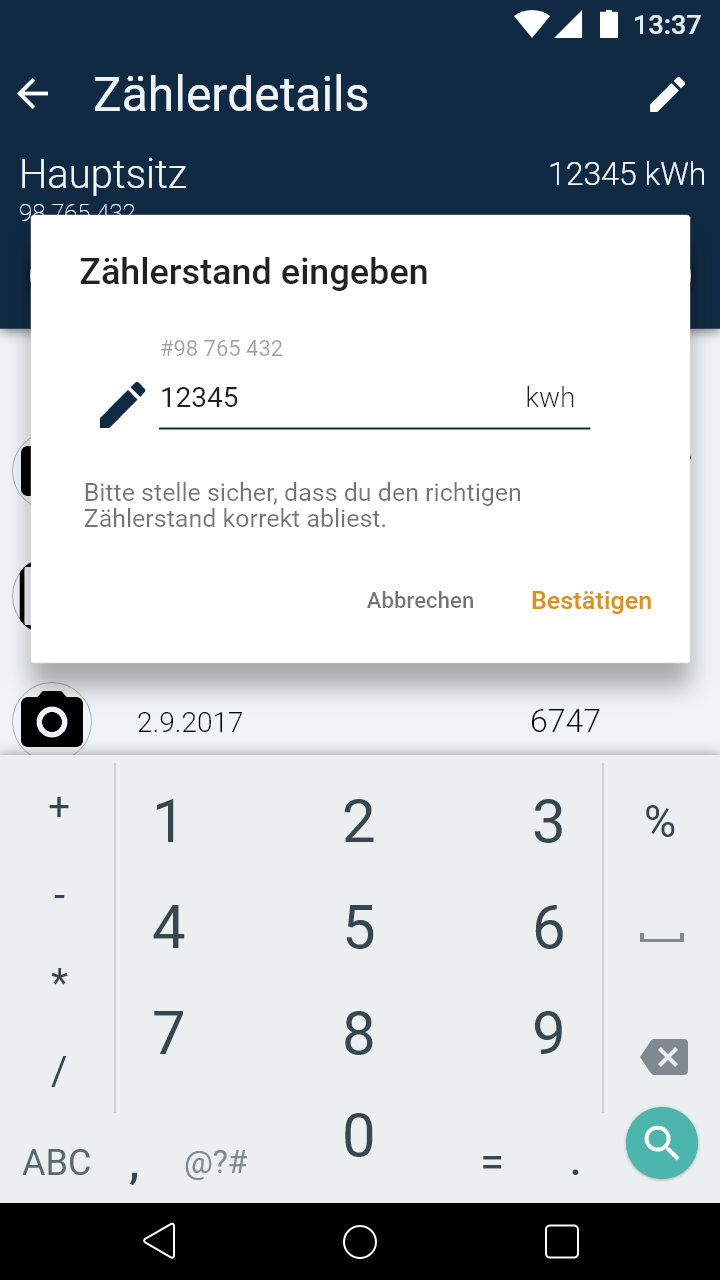
\includegraphics[scale = 0.22]{img/AndroidMockup/manuelEntry}		
	\caption{Manuelle Eingabe des Zählerstandes}
	\label{fig:mock-pw}
\end{figure}

\begin{figure}[h]
	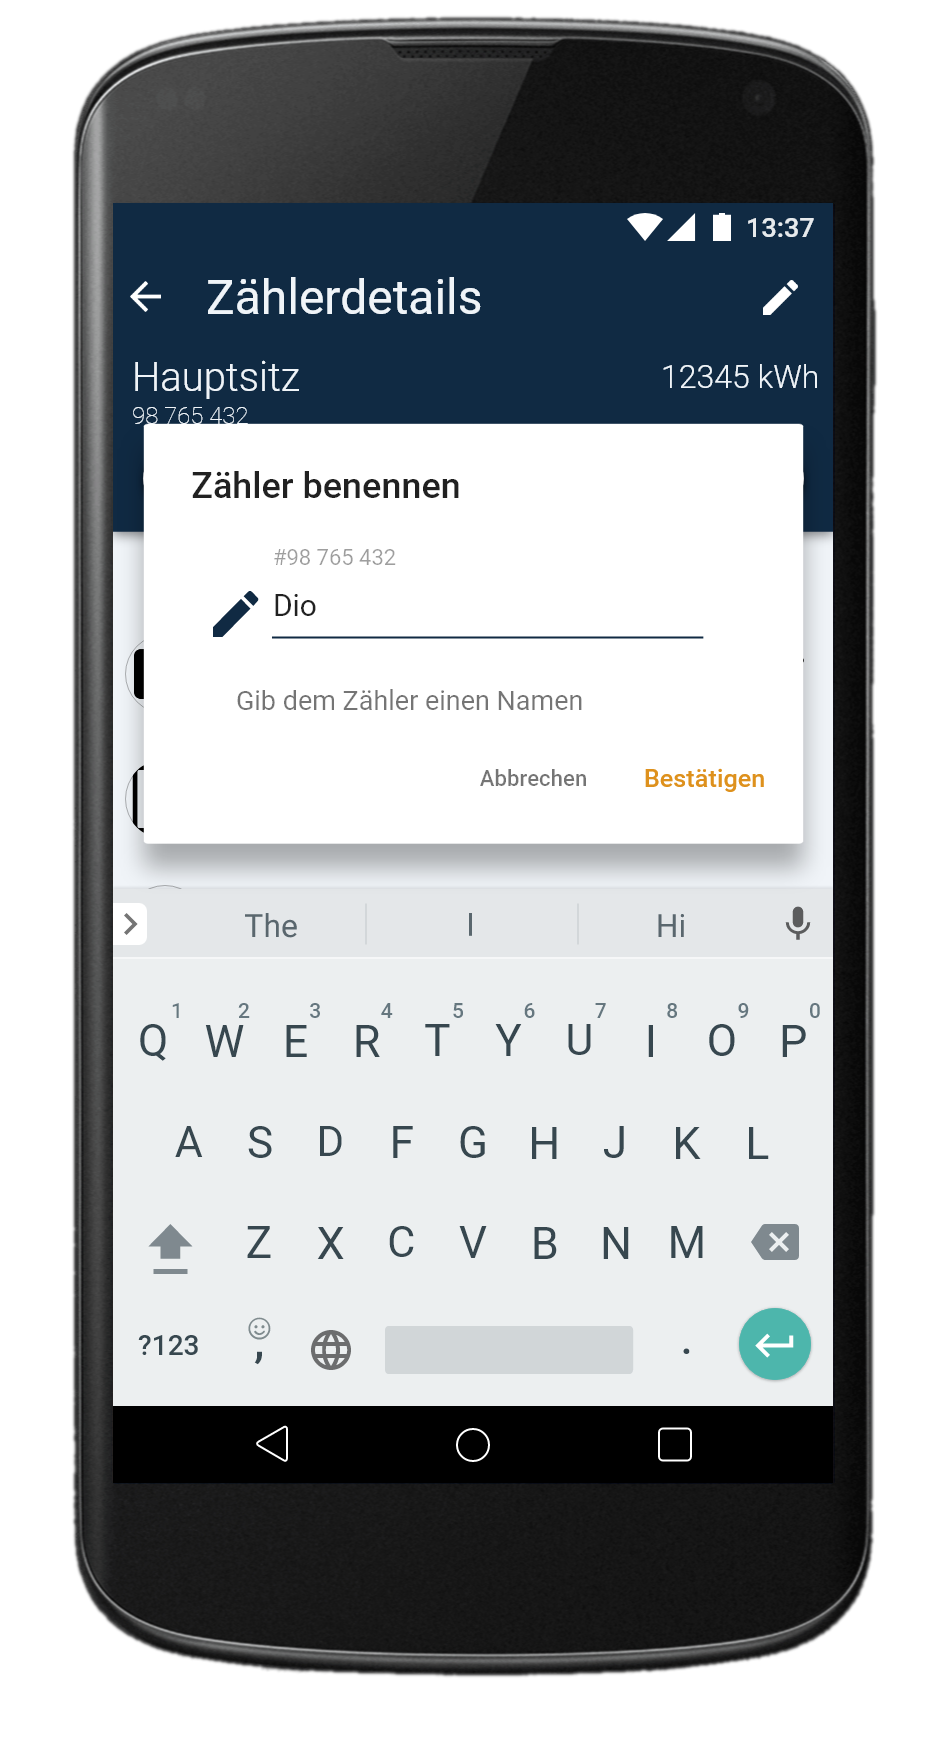
\includegraphics[scale = 0.22]{img/AndroidMockup/rename}		
	\caption{Netzwerkfehler}
	\label{fig:mock-pw}
\end{figure}

\begin{figure}[h]
	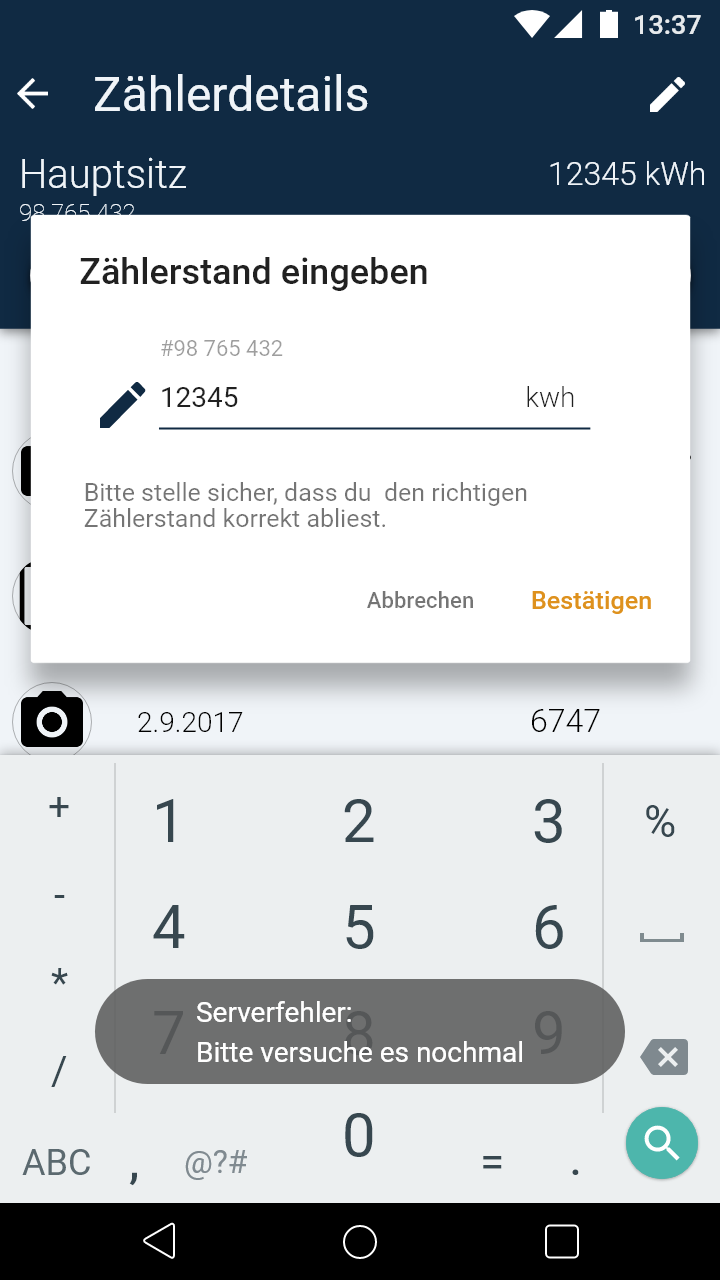
\includegraphics[scale = 0.22]{img/AndroidMockup/serverException}		
	\caption{Serverfehler}
	\label{fig:mock-pw}
\end{figure}

\begin{figure}[h]
	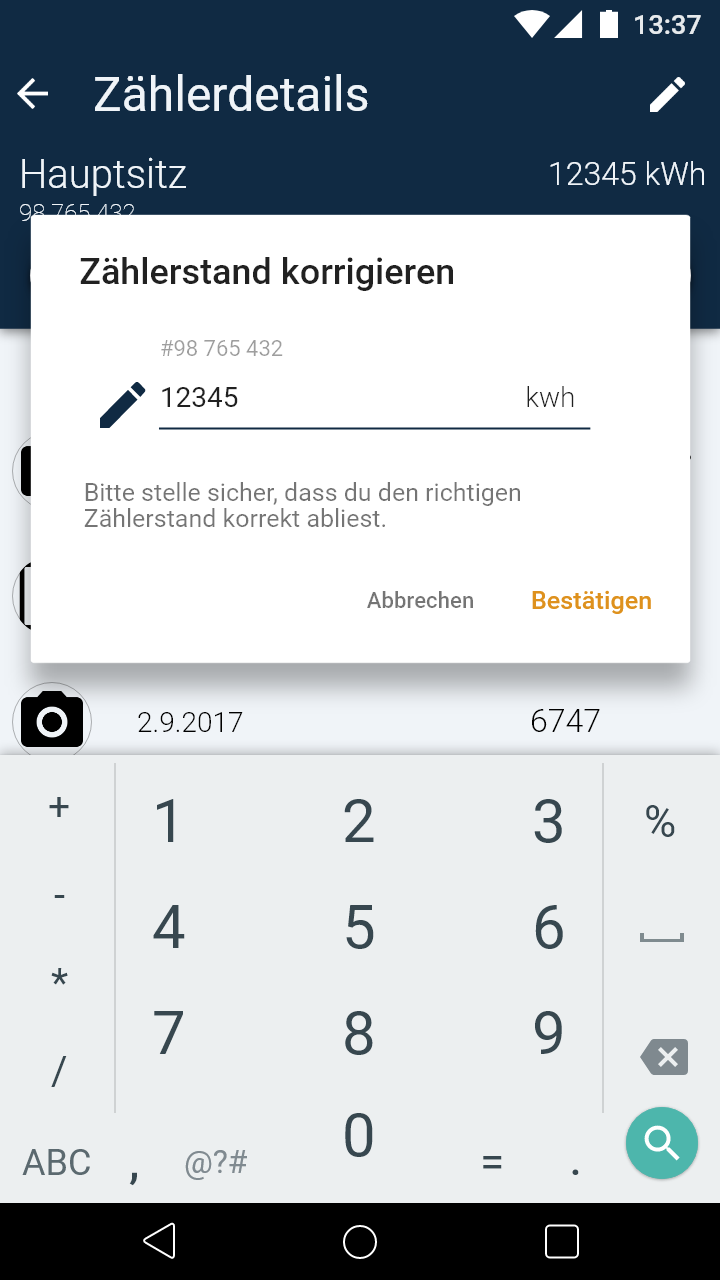
\includegraphics[scale = 0.22]{img/AndroidMockup/correct}		
	\caption{Zählerstand korregieren}
	\label{fig:mock-pw}
\end{figure}

\begin{figure}[h]
	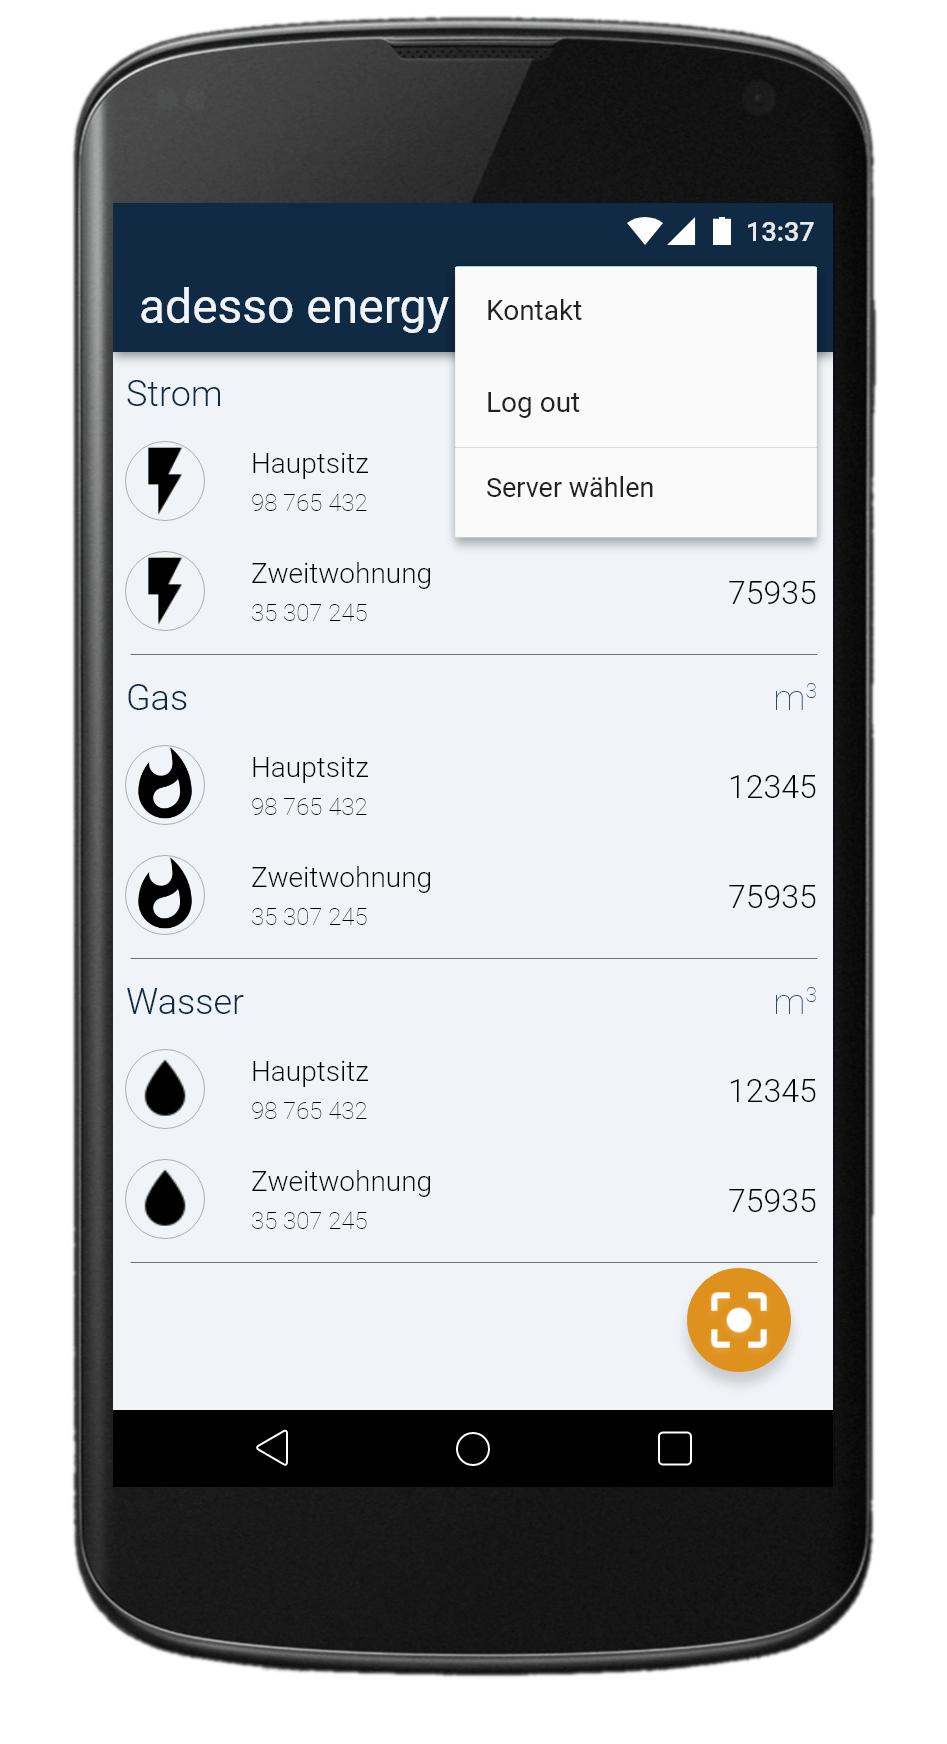
\includegraphics[scale = 0.22]{img/AndroidMockup/dropdown}		
	\caption{Dropdown Menü}
	\label{fig:mock-pw}
\end{figure}

\begin{figure}[h]
	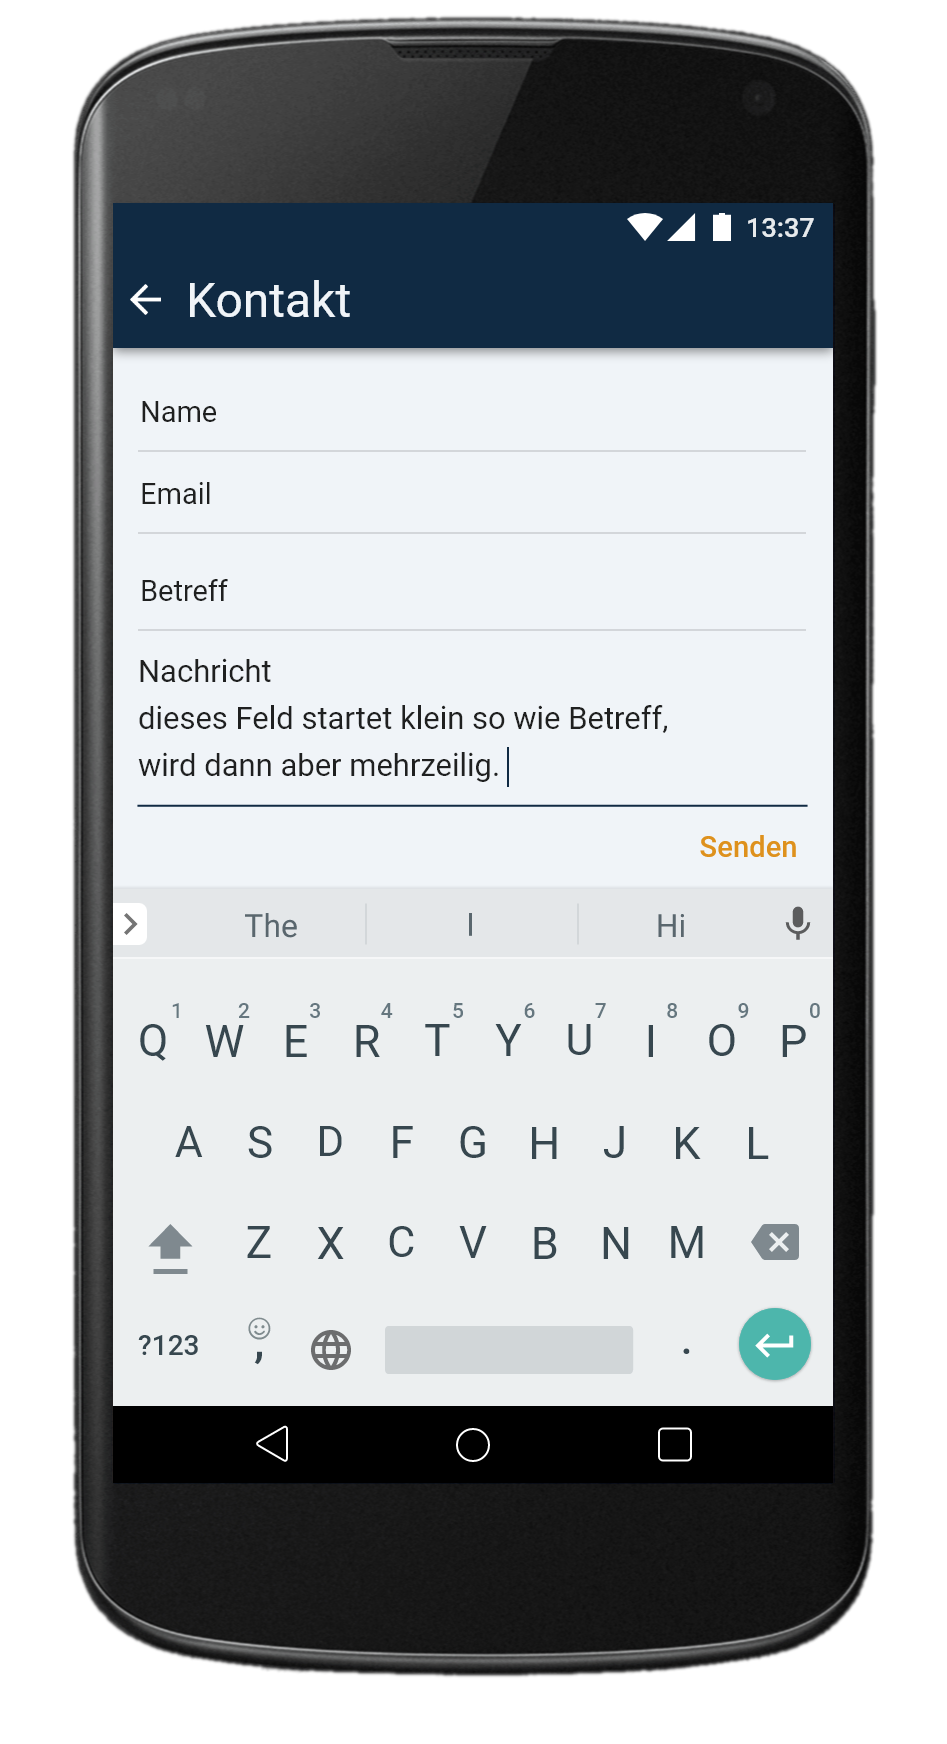
\includegraphics[scale = 0.22]{img/AndroidMockup/contact}		
	\caption{Kontakt Anfrage}
	\label{fig:mock-pw}
\end{figure}

\begin{figure}[h]
	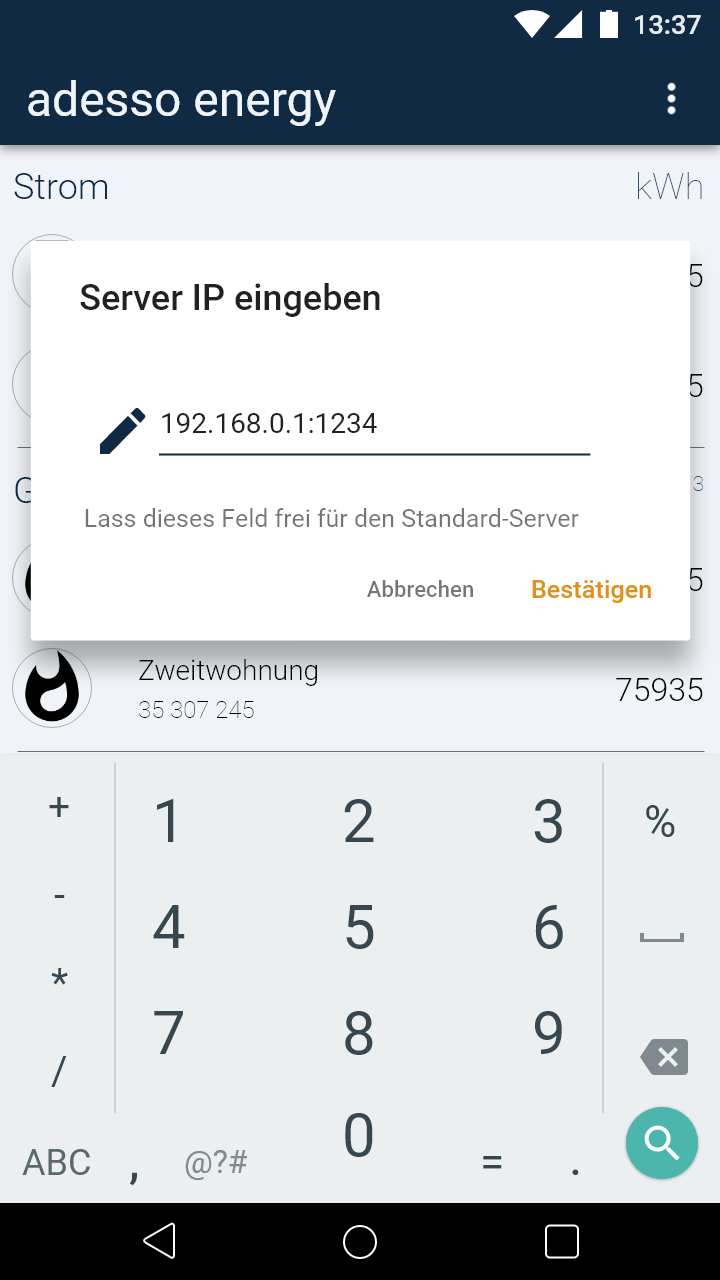
\includegraphics[scale = 0.22]{img/AndroidMockup/serverLocation}		
	\caption{Server Lokation ändern}
	\label{fig:mock-pw}
\end{figure}

